\section{Calculation method}
\label{sec:used_method}

\subsection{Survey and comparison of available methods}

In our simulation, we numerically solve the time-dependent Schrödinger equation.
There are multiple available algorithms for this task.
A widely used category of solving strategies are the \acrfull{fdtd} methods.
This approach is also widely adopted to simulate the solution of Maxwell equations \cite{maxwell1865, Ulf2001}.
\acrfull{fdtdq} however exhibit numerical instability \cite{Soriano2004}.
After a longer sequence of simulation steps, the solutions diverge.
There are various alterations to the basic method.
One such method was proposed by Min Zhu et al. \cite{Zhu2014} in the year 2014.
Their algorithm is called the \acrfull{rkhofdtd}.
In 2021, a follow-up paper \cite{Zhu_Wang_2021} demonstrated the superiority of \acrshort{rkhofdtd} over the basic \acrshort{fdtdq} approach.
In the same year, Frederick Ira Moxley et al. \cite{MOXLEY20122434} proposed another method based on \acrshort{fdtdq}.
These methods solve the majority of problems related to \acrshort{fdtdq}.

However, in our work, we use a different approach.
Back in 1982, D Kosloff and R Kosloff proposed a method \cite{KOSLOFF198335} to solve the time-dependent Schrödinger equation efficiently using Fourier transformation.
The advantage of this algorithm is the high numerical stability of the time evolution step.
In the adopted \acrshort{fft} method, no signs of divergence are present even after a large number of simulation steps.
The time development step of the algorithm has a time complexity of $\mathcal{O}(N\log N)$ since it only uses six \acrshort{fft} runs ($\mathcal{O}(N\log N)$ each) and three element-wise multiplication between tensors ($\mathcal{O}(N)$ each).
The amount of \acrshort{fft} runs and multiplications can be reduced further if we do not want to read the results of the time development in each step.
A significant speed-up can be reached by using a parallelized implementation of the \acrshort{fft} algorithm as we did by using an efficient \acrshort{gpu} implementation.

\subsection{Detailed explanation of the split-time Fourier method}

In the following part, we would like to explain the \acrshort{fft} method in detail.
Let us start by deriving the formal solution of the \ref{eq::schrodinger_general} differential equation.
\begin{equation}
	\label{eq:formal_solution}
	\begin{split}
		\int_{t_0}^t \frac{d}{d\tau}\Psi(\vec{r}, \tau) \; d\tau &= \int_{t_0}^t -\frac{i}{\hbar}\hat{H}\Psi(\vec{r}, \tau)\; d\tau\\
		\Psi(\vec{r}, t) - \Psi(\vec{r}, t_0) &= \int_{t_0}^t -\frac{i}{\hbar}\hat{H}\Psi(\vec{r}, \tau)\; d\tau\\
		&\;\:\vdots\\
		\Psi(\vec{r}, t) &= e^{-\frac{i}{\hbar}\hat{H}(t - t_0)} \Psi(\vec{r}, t_0)
	\end{split}
\end{equation}
where $\Psi(\vec{r}, t_0)$ is a specified initial state and $\Psi(\vec{r}, t)$ is the state after some $\delta t = t - t_0$ time.
The problematic part is the Hamiltonian operator in the exponent.
The kinetic and potential operators can not be commuted in general. Hence, exponential can not be factored.
We can decomposes the exponential by the symmetrical unitary product \cite{Fleck1976, FEIT1982412} as shown in the form \ref{eq:unitary_product}.
\begin{equation}
	\label{eq:unitary_product}
	e^{-\frac{i}{\hbar}\hat{H}\delta t} = e^{-\frac{i}{\hbar}(\hat{K} + \hat{V})\delta t} \approx e^{-\frac{i}{\hbar}\hat{K}\delta t / 2}\; e^{-\frac{i}{\hbar}\hat{V}\delta t}\; e^{-\frac{i}{\hbar}\hat{K}\delta t / 2}
\end{equation}
The error of this approximation is $\mathcal{O}(\delta t^3)$; therefore, we have to be careful with selecting a small enough time resolution.
When the potential energy is localized, the $\hat{V}$ operator is a simple multiplication with $V(\vec{r})$ function; thus the middle part of the product is as follows
\begin{equation}
	\label{eq:potential_prop}
	e^{-\frac{i}{\hbar}\hat{V}\delta t} \Psi = e^{-\frac{i}{\hbar}V(\vec{r})\delta t} \Psi
\end{equation}
The $\hat{K}$ kinetic operator involves calculating the spatial derivative of the wave function.

Previously in equation \ref{eq:derivative_of_wave_func} we have seen that calculating the spatial gradient $\nabla \Psi(\vec{r}, t)$ yields multiplication by $\frac{i}{\hbar}\vec{p} = i\vec{k}$.
We only need to get the value of the wave vector.
This is when the Fourier transform comes into play, which transforms between real space and momentum space.
The following relation holds for the derivative of an arbitrary $f$ function and its Fourier transform
\begin{equation}
	ik\mathcal{F}\{f\} = \mathcal{F}\{f'\}
\end{equation}
Taking the derivative in real space means multiplication by $ik$ imaginary wave number in momentum space.
We work with the $\Delta = \nabla \cdot \nabla$ Laplace operator, so we have to multiply by $(ik)^2 = -k^2$.
By exploiting the linearity of the Fourier transform, we arrive at the following formula for the kinetic energy part of the Hamiltonian function
\begin{equation}
	\label{eq:kinetic_op}
	\hat{K} \Psi = \frac{p^2}{2m}\Psi = -\frac{\hbar^2}{2m} \Delta \Psi = -\frac{\hbar^2}{2m}\mathcal{F}^{-1}
	\{
	-k^2\mathcal{F}\{\Psi\}
	\}
\end{equation}
where $\mathcal{F}^{-1}$ is the inverse Fourier transform. In momentum space, the $k$ wave number is trivially given as it can be thought of as the very coordinate the functions are parameterized with.
Having that said, it is essential to distinguish between $\nu$ frequency, $\lambda$ wavelength, $k$ wave number, and even $\omega$ angular velocity.
These relate as follows
\begin{equation}
	\label{eq:relation_of_dimensions}
	k = \frac{2\pi}{\lambda} = \frac{2\pi\nu}{v_{group}} = \frac{\omega}{v_{group}}
\end{equation}
where $v_{group}$ denotes the group velocity of the wave packet.

Actually, in equation \ref{eq:unitary_product}, the $\hat{K}$ kinetic energy operator is in the exponent multiplied by $-\frac{i}{\hbar}\delta t / 2$.
Using the knowledge gathered from equation \ref{eq:kinetic_op}, we can now write
\begin{equation}
	\label{eq:kinetic_prop}
	e^{-\frac{i}{\hbar}\hat{K}\delta t / 2}\Psi = \mathcal{F}^{-1}
	\left[
	e^{-\frac{i}{\hbar} \left(-\frac{\hbar^2}{2m}\right) \left(-k^2\right) \delta t / 2} \mathcal{F}\left[ \Psi \right]
	\right] = 
	\mathcal{F}^{-1}
	\left[
	e^{-\frac{i k^2 \hbar \delta t}{4m}} \mathcal{F}\left[ \Psi \right]
	\right]
\end{equation}

Before writing the pseudo-code, let us write the wave function as a function of discrete $i_j \in \{0, 1, \dots, N_j - 1\}$ coordinates where $j \in \{x, y, z, t\}$ and $N_j$ are the number of discrete grid points along each axis.

Now $\vec{r}_x = i_x \delta x$, $\vec{r}_y = i_y \delta y$, $\vec{r}_z = i_z \delta z$ and $t = i_t \delta t$ are the original spatial and time coordinates and $\delta j$ is the resolution of the different dimensions respectively.
With the new discretized coordinates, the Schrödinger equation \ref{eq::schrodinger_general} can be written in the following form
\begin{equation}
	\label{eq:discretized_schrodinger}		
	i \hbar \frac{d}{dt}\Psi(i_x, i_y, i_z, i_t) = - \frac{\hbar^2}{2m}\Delta\Psi(i_x, i_y, i_z, i_t) + V(\vec{r})\Psi(i_x, i_y, i_z, i_t)
\end{equation}
Having a discrete data set, \acrfull{dft} can be efficiently implemented using the \acrfull{fft} algorithm.
The output of the simulation is the wave function.
The probability density can be obtained by calculating the square of the absolute value of the wave function for each grid cell which is the same as calculating the standard scalar product between $\bra{\Psi}$ and $\ket{\Psi}$ vectors where $\bra{\Psi}$ is the transposed complex conjugate of $\ket{\Psi}$ as seen in equation~\ref{eq:probability_density}.
\begin{equation}
	\label{eq:probability_density}
	p(\vec{r}, t) = |\Psi(\vec{r}, t)|^2 = \braket{\Psi(\vec{r}, t)}
\end{equation}
Making use of formulas \ref{eq:unitary_product}, \ref{eq:potential_prop} and \ref{eq:kinetic_prop} and plugging them into the formal solution of the Schrödinger equation we can create an algorithm for the time development of the wave function.
We will use the $\Psi$ to represent a complex-valued tensor where the elements of this tensor can be obtained by using the $i_j$ discrete indices.
The algorithm can be written in the form of the following pseudo code
\begin{algorithm}
	\caption{Time advance algorithm}\label{alg:time_advance}
	\begin{algorithmic}
		\State $ \Psi \gets $ initial state of the wave function
		\State $ V \gets $ localized potential
		\State $ \delta t \gets $ time resolution
		\State $ N_t \gets $ number of time steps
		\For{$i \in [0, N_t)$}
		\State $\Psi^{(1)} \gets FFT^{-1}
		\left[
		P_K\; FFT\left[ \Psi \right]
		\right]
		$
		
		\State $\Psi^{(2)} \gets P_V\; \Psi^{(1)}$
		
		\State $\Psi \gets FFT^{-1}
		\left[
		P_K\; FFT\left[ \Psi^{(2)} \right]
		\right]
		$
		\State Visualize $|\Psi|^2$
		\EndFor
	\end{algorithmic}
\end{algorithm}

Here $P_K(i_x, i_y, i_z) \sim e^{-\frac{i \hbar \delta t}{4m} \left[(2\pi i_x / N_x / \delta x)^2 + (2\pi i_y / N_y /\delta y)^2 + (2\pi i_z / N_z / \delta z)^2\right]}$ is the kinetic energy propagator in momentum space and $P_V(i_x, i_y, i_z) = e^{-\frac{i}{\hbar}V(i_x, i_y, i_z)\delta t}$ is the potential energy propagator in real space.
We used the discretized coordinates to express the same operations as in \ref{eq:potential_prop} and \ref{eq:kinetic_prop}.
Please note that in the kinetic propagator's case, it is important to follow the convention used by the specific \acrshort{fft} implementation.
The formula written here is not entirely correct.
The \acrshort{fft} used in our implementation puts the amplitude associated with the largest representable frequency of $\frac{1}{2N}$ in the middle of the tensor.
In the second half of the tensor for each axis, the amplitudes are for the negative frequencies in ascending absolute value so that the largest index represents the $-\frac{1}{N}$ frequency.
This means that we had to modify the definition of $P_K$ accordingly.
One way to make the correction is to check whether $i_j / N_j > \frac{1}{2}$ is true. If it is, then modify it like $i_j := N - i_j$.

\subsection{Defining Gaussian wave packets}

In the algorithm, first, we have to specify an initial state for the wave function.
Erwin Schrödinger introduced the concept of the \acrfull{wp}.
A \acrshort{wp} is a wavefront that propagates and reflects as a classical particle would do
and also exhibits all the wave-like behavior described by \acrshort{qm}.
It bridges the gap between classical and quantum physics.
The term \acrfull{wpd} refers to the process of modeling \acrshort{qm} systems by initializing \acrshort{wp}s
and observing the propagation, reflection scattering, and interference of the \acrshort{wp}.
In our work, we use Gaussian \acrshort{wp}s.
This probability density of this \acrshort{wp} has Gaussian distribution \cite{Zhang2010}, hence the name.
The definition of such a packet can be written in the following form
\begin{equation}
	\label{eq:gaussiaon_wp}
	\psi(\vec{r};\; a, \vec{r_0}, \vec{k_0}) = \left( \frac{2}{\pi a^2} \right)^{\frac{D}{4}} \cdot exp\left( i\vec{k_0} \cdot \vec{r} \right) \cdot exp \left( -\frac{|\vec{r} - \vec{r_0}|^2}{a^2} \right)
\end{equation}
where $\vec{r_0}$ is the initial position (with the highest probability density), $\vec{k_0}$ is the initial wave vector, and $D$ is the dimension, which is  $D:=3$ in our simulation.
We can obtain the width of the Gaussian \acrshort{wp} as $\Delta r = \frac{a}{2}$.

\subsection{A simple trick to optimize the algorithm}

If we do not want to visualize the probability density in each iteration, we can further optimize the calculation by merging the first step of the $n$th iteration and the last step of the $(n-1)$th iteration.
If we omit the visualization step, we can do one forward \acrshort{fft} then perform a multiplication between the moment space wave tensor and the $P_K^2$ kinetic propagator calculated for a whole $\delta t$ interval --instead of the one used in Algorithm \ref{alg:time_advance} calculated for $\delta t / 2$ interval-- then do the backward \acrshort{fft}.
The pseudo-code of this optimized algorithm is written below
\begin{algorithm}
	\caption{Optimized time advance algorithm without visualization}\label{alg:time_advance_optimized}
	\begin{algorithmic}
		\State $ \Psi \gets $ initial state of the wave function
		\State $ V \gets $ localized potential
		\State $ \delta t \gets $ time resolution
		\State $ N_t \gets $ number of time steps
		\For{$i \in [0, N_t)$}
		\State $\Psi^{(1)} \gets FFT^{-1}
		\left[
		P_K^2\; FFT\left[ \Psi \right]
		\right]
		$
		\State $\Psi^{(2)} \gets P_V\; \Psi^{(1)}$		
		\EndFor
	\end{algorithmic}
\end{algorithm}

\subsection{Free space boundary condition}

When working with \acrshort{dft} it is vital to take into account the boundary conditions of the transformed region.
The \acrshort{dft} implies a periodic boundary condition in which value at $i_j = 0$ connects smoothly to values at $i_j = 0$ for each of the respective $j \in \{x, y, z\}$ dimensions.
If the data transform does not satisfy this condition, unrealistic artifacts arise.
One technique to battle this requirement is to define a high potential wall on all the edges of the simulated volume so that the wave packet bounces back and never reaches the problematic edge.
This, however, limits the possible simulation cases since we can not simulate scenarios where the wave packet would leave the volume.
The wave packet reflected by the boundary potential interferes with itself, thus potentially disturbing the observation of the object of simulation.
In our implementation, we used another approach called free space boundary condition.
This fixes the issues arising from the periodic boundary condition and the potential box.
We extend the simulated volume beyond the observed part and outside the visible box, and we create a draining potential.
This draining potential gradually increases towards the edge of the simulated volume.
As the name suggests, its effect on the wave packet is that it diminishes its amplitude.
By initializing a high enough draining potential, the unrealistic artifacts on the edge of the simulated volume are practically negligible.
In equation \ref{eq:potential_prop}, we have seen that the potential propagator is a multiplication by a unit length complex number with phase proportional to $V(\vec{r})$ localized potential.
This normally only introduces a rotation on the complex plane.
We can, however incorporate the desired draining effect by introducing complex potential.
Let us examine what happens if a complex number has a complex phase!
\begin{equation}
	\label{eq:complex_phase}
	e^{i |z|e^{i\gamma}} = e^{i|z|\left[cos(\gamma) + isin(\gamma)\right]} = e^{i|z|cos(\gamma) - |z|sin(\gamma)}
	= e^{i|z|cos(\gamma)}e^{-|z|sin(\gamma)}
\end{equation}
In equation \ref{eq:complex_phase}, we showed that by defining an imaginary potential, we can reduce the magnitude of the wave function if we then apply the potential propagator.
In our simulation, we initialized the draining potential to be zero in the observed region, and right from the corners of this box, it begins to increase as a quadratic function of distance from the center of the simulated volume.
It reaches its maximum in the four corners of the simulated volume.
\begin{figure}[hbt!]
	\centering
	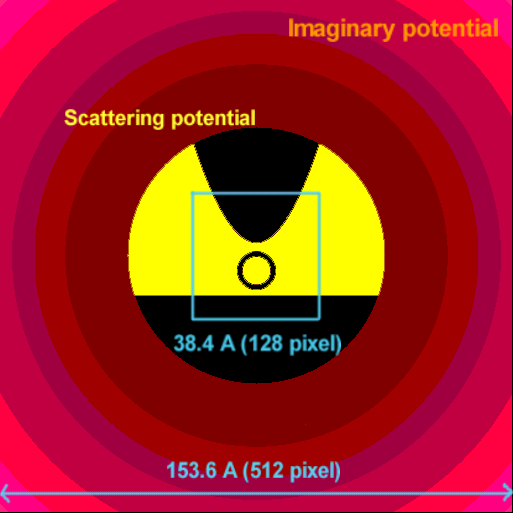
\includegraphics[width=0.4\textwidth]{figures/REGIONS.png}
	\caption{Calculation scheme used for the simulation of a \acrfull{stm} investigation of a carbon nanotube [hivatkozás az
		1998-as PRB cikkre]. The upper black ellipse is the STM tip, the middle
		black ring is the cross-section of the nanotube, and the lower black
		region is the support electrode. The red concentric circles show the
		imaginary potential with increasing magnitude.}
	\label{fig:draining_potential}
\end{figure}

